\chapter{\IfLanguageName{dutch}{Stand van zaken}{State of the art}}
\label{ch:stand-van-zaken}

% Tip: Begin elk hoofdstuk met een paragraaf inleiding die beschrijft hoe
% dit hoofdstuk past binnen het geheel van de bachelorproef. Geef in het
% bijzonder aan wat de link is met het vorige en volgende hoofdstuk.

% Pas na deze inleidende paragraaf komt de eerste sectiehoofding.

%Dit hoofdstuk bevat je literatuurstudie. De inhoud gaat verder op de inleiding, maar zal het onderwerp van de bachelorproef *diepgaand* uitspitten. De bedoeling is dat de lezer na lezing van dit hoofdstuk helemaal op de hoogte is van de huidige stand van zaken (state-of-the-art) in het onderzoeksdomein. Iemand die niet vertrouwd is met het onderwerp, weet nu voldoende om de rest van het verhaal te kunnen volgen, zonder dat die er nog andere informatie moet over opzoeken \autocite{Pollefliet2011}.

%Je verwijst bij elke bewering die je doet, vakterm die je introduceert, enz. naar je bronnen. In \LaTeX{} kan dat met het commando \texttt{$\backslash${textcite\{\}}} of \texttt{$\backslash${autocite\{\}}}. Als argument van het commando geef je de ``sleutel'' van een ``record'' in een bibliografische databank in het Bib\LaTeX{}-formaat (een tekstbestand). Als je expliciet naar de auteur verwijst in de zin, gebruik je \texttt{$\backslash${}textcite\{\}}.
%Soms wil je de auteur niet expliciet vernoemen, dan gebruik je \texttt{$\backslash${}autocite\{\}}. In de volgende paragraaf een voorbeeld van elk.

%\textcite{Knuth1998} schreef een van de standaardwerken over sorteer- en zoekalgoritmen. Experten zijn het erover eens dat cloud computing een interessante opportuniteit vormen, zowel voor gebruikers als voor dienstverleners op vlak van informatietechnologie~\autocite{Creeger2009}.

%-----------------------------------
% BESPREKING ELLEN

%waar staat peru in ontwikkeling op vlak van ict
%digital gap
%duurzame ontwikkelingsdoelen agenda 2030 vn = SDG 
%17 logo's
%SDG --> ICT
%milenium doelstellingen 2015
%
%peru in het algemeen
%als ontwikkelingsland --> vn/SDG
%hegt onderwijs in peru
%ict 
%digital gab 
%projecten in het verleden/organisaties ict hulp?
%
%
%vlirous - project beurs - peru project -computers recycleren

\section{Peru: een bloemlezing}
In dit hoofdstuk worden verschillende kenmerken van het land Peru besproken. 
\subsection{Geografisch}
Peru ligt aan de westkust van zuid-Amerika. Het grenst in het noorden aan Colombia en Ecuador, in het oosten aan Bolivia en Brazilië en in het zuiden aan Chili. Aan de westkust van het land ligt de Grote Oceaan. Lima is de hoofdstad van het land, en telt ruim 10 miljoen inwoners. Qua oppervlakte is Peru 42 keer zo groot als België, het meet ongeveer 1.285.216 km\textsuperscript{2}. 

\subsubsection{Landschap}
Peru bestaat uit 3 verschillende landschapssoorten: het kustgebied, de bergen en de jungle. De kust van Peru bestaat uit woestijn die tussen de zee en de bergen ligt. De bergen bestaan vooral uit het Andes gebergte, en daarachter ligt de jungle. Die kan opgesplitst worden in 2 verschillende stukken. Er is het hoge regenwoud, dat op 700 meter hoogte ligt en de amazone jungle waar de Amazone rivier door stroomt. \autocite{ToPeru2020}

\subsection{Demografisch}
Peru heeft op dit moment 32 miljoen inwoners \autocite{Overheid2020}. Officieel worden er 3 talen gesproken: Spaans, Quechua en Aymara. Aymara is een taal die tot de familie van Aru behoort. Ze wordt gesproken door ongeveer 450.000 mensen. \autocite{CulturaPeru2020} Ze wordt ook gesproken in Bolivia en Noord-Argentinië en Chili. In de Amazone worden bijna 70 verschillende onofficiele, lokale talen gesproken. \autocite{dosmanosperu}

\subsection{Cultuur en Economie}
De nationale feestdag van Peru valt op 28 Juli. In Peru worden deze dagen de Fiestas Patrias genoemd. \autocite{dosmanosperu2018}  Verder wordt er in Peru betaald met de Peruviaanse sol. Op dit moment is 1 euro ongeveer gelijk aan 3,82 Peruviaanse sol.

\section{Peru als ontwikkelingsland}
\subsection{Wat is een ontwikkelingsland?}
Volgens het volgend boek, \autocite{MarcJ.Bossuyt2005}, bestaat er geen algemene definitie voor een ontwikkelingsland. Dat komt omdat de verschillende internationale instellingen, die zich bezig houden met het quoteren van landen, verschillende criteria gebruiken. Daarnaast is het soms niet duidelijk wat er met ontwikkeling bedoeld wordt.
De status van een ontwikkelingsland is niet permanent, een land kan zich verder ontwikkelen.

\subsection{Indeling van ontwikkelingslanden}
De indeling van ontwikkelingslanden kan op 2 manieren gedaan worden. De eerste is door middel van abstracte criteria, de tweede door middel van lijsten. Een abstract criterium wordt op alle landen gelijk toegepast. Alle landen die onder een vooraf bepaalde grens vallen zijn dan ontwikkelingslanden, de anderen ontwikkelde landen. Een lijst is een volledige opsomming, van items die gebaseerd zijn op onbetrouwbare of onbestaande statistieken, waaraan een land moet voldoen. \autocite{MarcJ.Bossuyt2005},

In het "World Economic Situation and Prospects 2019" rapport \autocite{unitednations2019} deelt de  Verenigde Naties alle landen in 3 grote groepen op. Volgens de VN zijn er 43 ontwikkelde landen, 17 landen die de overgang maken tussen onderontwikkeld, en ontwikkeld land en maar liefst 127 landen die als onderontwikkeld worden beoordeeld. België behoort tot de ontwikkelde landen, Peru tot de onderontwikkelde landen. \autocite{unitednations2019}

De VN ontdekte dat deze verdeling niet perfect was. Ze konden niet alle ontwikkelingslanden over dezelfde kam scheren, omdat er landen waren die soms meer aandacht verdienden dan anderen op vlak van internationale ontwikkelingssamenwerking. De VN stelde naast ontwikkelde, landen in overgang en onderontwikkelde landen, nog 3 andere groepen op, om de onderontwikkelde landen in op de delen: 

\begin{itemize}
\item De minst ontwikkelde landen, (least developed country's of LDC);
\item De ontwikkelingslanden zonder zeekust, (landlocked developing country's of LLDC);
\item de kleine eilandstaten in ontwikkeling, (Small island developing states of SIDS).
\end{itemize}
\autocite{MarcJ.Bossuyt2005},

Een land kan tot meerdere categorieën behoren. De lijsten wordt elke 3 jaar door ECOSOC (United Nations Department of Economic and Social Affairs) in de verschillende groepen opgedeeld. In 2018 deed ECOSOC dat, en waren er 47 LDC's, 31 LLDC's en 48 SIDS. Peru behoort niet tot een van deze groepen. \autocite{MarcJ.Bossuyt2005},

\subsection{Human development index}
De human development index geeft landen een score. Dit gebeurd door elk land te quoteren op vlak van verschillende dimensies. De quoteringsvlakken die in acht worden genomen zijn de onderwijsdimensie, de gezondheidsdimensie en de levensstandaard dimensie.

De gezondheidsdimensie wordt beoordeeld aan de hand van de levensverwachting bij de geboorte. De onderwijsdimensie wordt gemeten aan de hand van het aantal verwacht aantal schooljaren voor volwassenen van 25 jaar en verwachte schooljaren voor schoolgaande kinderen. Tot slot wordt de levensstandaard dimensie gemeten aan de hand van het bruto nationaal inkomen per inwoner. De HDI werd gemaakt om te benadrukken dat mensen en hun capaciteiten de ultieme criteria moeten zijn voor het beoordelen van de ontwikkeling van een land, en niet alleen economische groei. \autocite{UNDP2019}

Met de scores die resulteren uit de berekening, kan een rangschikking gevormd worden. Die rangschikking kan dan duiden op welk land beter ontwikkeld tegenover andere landen. 

Sinds 1990 heeft het Ontwikkelingsprogramma van de  Verenigde Naties (UNDP) in zijn zijn jaarlijkse Human Development Reports, de Human development index voor elk van zijn land gepubliceerd. \autocite{AmbujD.Sagar1997} Deze index is belangrijk alternatief voor de traditionele eendimensionale maatstaf voor ontwikkeling (BBP). 

België stond in 2019 op de 17de plaats, Peru op de 82ste. Bovenaan de lijst trimfeert Noorwegen. \autocite{UNDP2019a} 

\subsubsection{Kritiek op de HDI}
Er kwam kritiek op de indicator aangezien hij enkel sociale factoren in rekening brengt. Sinds 2010 gebruikt de VN een aangepaste versie van de indicator: de index van duurzame menselijke ontwikkeling (HSDI) die ook de koolstofemissies per capita in rekening brengt. \autocite{Economie2018}

\section{Ontwikkelingshulp}

\subsection{Verenigde Naties}
De Verenigde Naties is een internationale organisatie die in 1945 is opgericht. De organisatie bestaat momenteel uit 193 lidstaten. Zowel België als Peru werden in 1945 lid van de  Verenigde Naties. De Verenigde Naties heeft een handvest dat werd ondertekend op 26 juni 1945, in San Francisco. Het handvest trad in werking op 24 oktober 1945.Vanwege de bevoegdheden in het handvest en het unieke internationale karakter, kunnen de  Verenigde Naties actie ondernemen tegen de problemen waarmee de mensheid in de 21e eeuw wordt geconfronteerd, zoals vrede en veiligheid, klimaatverandering, duurzame ontwikkeling, mensenrechten, ontwapening, terrorisme, humanitaire hulp en noodsituaties op gezondheidsgebied, gendergelijkheid, bestuur, voedselproductie en meer. \autocite{Nations2020}

Op 1 januari 2017 volgde de Portugese socialistische politicus António Guterres, Ban Ki-moon op als Secretaris-generaal van de organisatie. 

De belangrijkste organen van de VN zijn de Algemene Vergadering, de Veiligheidsraad, de Economische en Sociale Raad, de trustschapsraad, het Internationaal Gerechtshof en het VN-secretariaat. Ze werden allemaal opgericht in 1945 toen de VN zelf werd opgericht. 

De VN bestaat uit vele programma's, fondsen en gespecialiseerde organisaties, allemaal met hun eigen leiderschap en budget. Een aantal bekende zijn Unicef, het Internationaal monetair fonds (IMF), Unesco, de wereld gezondheid (WHO). Natuurlijk bestaan er nog vele anderen. In dit onderzoek zal vooral het  Verenigde Naties ontwikkelingsprogramma (UNDP) aan bod komen. Zoals de naam doet vermoeden houd dit deel van de  Verenigde Naties zich bezig met ontwikkelingshulp.

\subsubsection{UNDP: Het Verenigde Naties ontwikkelingsprogramma}
Zoals eerder vermeld helpt de Verenigde Naties mee aan ontwikkelingshulp. Dit doen ze via een apart programma, het United Nations Development Programme (UNDP). Het ontwikkelingsprogramma van de  Verenigde Naties is het wereldwijde ontwikkelingsnetwerk van de VN en pleit voor verandering. Het verbindt landen met kennis, ervaring en middelen om mensen te helpen een beter leven op te bouwen UNDP werkt in 170 ongeveer landen en gebieden, draagt bij tot de uitroeiing van armoede en gaat de ongelijkheden en uitsluiting tegen. Ze helpen de landen bij het ontwikkelen van hun ontwikkelingsbeleid, leiderschapsvaardigheden, partnerschap mogelijkheden, institutionele capaciteiten en het opbouwen van veerkracht om betere ontwikkelingsresultaten te bekomen. \autocite{DevelopmentProgram2020}
Hun werk is geconcentreerd op drie belangrijke aandachtsgebieden:

\begin{enumerate}
\item Duurzame ontwikkeling
\item Democratisch bestuur en vredesopbouw
\item Klimaat- en rampenbestendigheid
\end{enumerate}

 Jaarlijks brengt UNDP een Human Development Report uit. Dat concentreert zich op het mondiale debat over belangrijke ontwikkelingskwesties en biedt nieuwe meetinstrumenten, innovatieve analyses en vaak controversiële beleidsvoorstellen. \autocite{DevelopmentProgram2020} 

\subsubsection{UNDP Strategic Plan}
Het Strategisch Plan (2018-2021) van UNDP is ontworpen om te reageren op de grote diversiteit van de landen die ze bedienen. Deze diversiteit wordt weerspiegeld in drie brede ontwikkelingscontexten: \autocite{DevelopmentProgram2020}

\begin{enumerate}
\item Roei armoede uit in al zijn vormen en dimensies
\item Versnel structurele transformaties
\item Bouw veerkracht op tegen schokken en crises
\end{enumerate}

Om deze brede doelen te bereiken heeft UNDP een reeks benaderingen opgesteld die ze hun "Signature Solutions" noemen:

\begin{enumerate}
	\item Mensen uit armoede houden
	\item Een bestuur een vreedzame, rechtvaardige en inclusieve samenlevingen
	\item Crisispreventie en verhoogde veerkracht
	\item milieu : natuurgebaseerde oplossingen voor ontwikkeling
	\item Schone, betaalbare energie
	\item Empowerment van vrouwen en gender gelijkheid
\end{enumerate}

\subsubsection{UN Capital Development Fund}
UNDP beheert ook het UN Capital Development Fund. Dat is een fonds dat ontwikkelingslanden helpt hun economie te laten groeien door bestaande bronnen van kapitaalhulp aan te vullen door middel van subsidies, leningen en VN-vrijwilligers. De vrijwilligers zijn met meer dan 6.500, die 160 landen vertegenwoordigen. Ze ondersteunen 38 VN-partners op vlak van vrede, veiligheid, mensenrechten, humanitaire hulpverlening en ontwikkeling via wereldwijd vrijwilligerswerk.

\subsection{De millenniumdoelstellingen}
Op de website van 11-11-11 staat het volgende te lezen over de millenniumdoelstellingen: "In september 2000 verzamelden alle staatshoofden en regeringsleiders van de VN-lidstaten in het hoofdkwartier in New York voor de eerste Algemene Vergadering van het nieuwe millennium. Aan het einde van de driedaagse ondertekenden de leden unaniem de Millenniumverklaring. Deze verklaring bevatte een reeks becijferde en in de tijd geplande doelen: de Millenniumdoelstellingen." \autocite{11.11.112019}

Verder staat er te lezen: "Ruw samengevat gaat het bij de eerste 7 Millenniumdoelstellingen om opdrachten die een betere menselijke ontwikkeling in het Zuiden voor ogen hebben. De landen moeten die zelf realiseren. Deze doelstellingen zijn gekwantificeerd en kennen een tijdslimiet. Millenniumdoelstelling 8, onder de titel "wereldwijd partnerschap", moet zorgen voor een internationaal beleid waardoor de eerste 7 opdrachten kunnen slagen. Van bij het begin was er discussie over de reikwijdte van de Millenniumdoelstellingen. Waren ze utopisch of net akelig pragmatisch?" \autocite{11.11.112019}

Volgens \autocite{Tjoa2016} kunnen de millenniumdoelstellingen worden beschouwd als een van de belangrijkste en succesvolle initiatieven om armoede in de moderne geschiedenis uit te bannen.

In Figuur \ref{milleniumdoelstellingen} worden de doelstellingen duidelijk weergegeven.

 
 \subsubsection{De verschillende doelstellingen}
 \begin{enumerate}
 \item Roei extreme armoede en honger uit
 \item Basisonderwijs voor alle kinderen
 \item Seksegelijkheid en mondige vrouwen
 \item Minder kindersterfte
 \item Verbeter de gezondheid van kraamvrouwen
 \item Bestrijd hiv en aids, malaria en andere dodelijke ziektes
 \item Een goed leefmilieu 
 \item Wereldwijde samenwerking
\end{enumerate}
\autocite{NOS2015}

\begin{figure}[h!]
	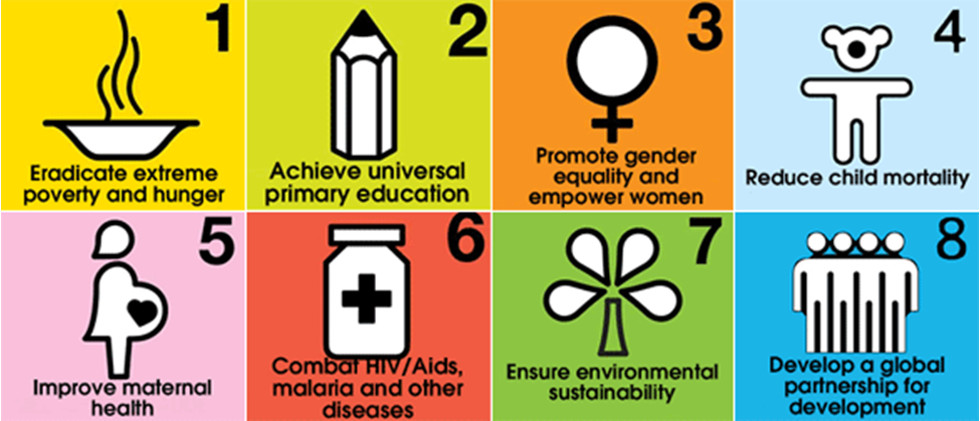
\includegraphics[width=\textwidth]{../img/millenniumdoelstellingen.jpg}
	\caption{De 8 millenniumdoelstellingen \autocite{NOS2015}}
	\label{milleniumdoelstellingen}
\end{figure}

 \subsubsection{ICT binnen de millenniumdoelstellingen}
 Op het eerste zicht is geen enkele doelstelling specifiek gericht op ICT. ICT kan bij vele doelstellingen een hulpmiddel zijn om die doelstelling te bereiken. Zo kon onder de achtste doelstelling, wereldwijde samenwerking, ICT een concretere functie innemen: ICT kan ervoor zorgen dat landen, en personen sneller kunnen communiceren. Het was een uitdaging, om in functie van wereldwijde samenwerking, ICT een boost te geven. Het gaat onder andere om ontwikkeling op vlak van internetaansluitingen, mobiele telefoons en andere ICT gerelateerde zaken. \autocite{NOS2015}
 
 \subsubsection{Algemene resultaten}
 De landen die zich engageerden hadden 15 jaar de tijd, om de doelstellingen te behalen. Op 31 december 2015 liepen de doelstellingen af.
 Een aantal doelstellingen had een positieve afloop, en bereikten hun vooropgestelde doel. Zo gaan bijna evenveel meisjes als jongens naar school, hebben meer mensen toegang tot drinkbaar water dan ooit en werd de extreme armoede gehalveerd. Ook op vlak van basisonderwijs, de strijd tegen hiv/aids en het terugdringen van kinder- en moedersterfte werd vooruitgang geboekt. Maar de vooruitgang van deze laatste doelstellingen was niet voldoende om de vooropgestelde doelen te behalen. \autocite{Tierens2014}

Deze resultaten zijn erg algemeen. Er wordt gesproken over algemene vooruitgang, en niet over welke landen of continenten meer vooruitgang boekten dan anderen. Zo boekte China een spectaculaire vooruitgang, maar hinken de regio's Sub-Sahara Afrika en West-Azië zwaar achterop. \autocite{Tierens2014}
 
 \subsubsection{Resultaten op vlak van ICT}
Over de vooruitgang op vlak van informatica stelt \autocite{Kampherbeek2012} het volgende: "Het aantal mobiele telefoons en internet aansluitingen is de laatste jaren ook in de ontwikkelingslanden flink gestegen. Het aantal unieke internetgebruikers is nu groter in ontwikkelingslanden dan in de ontwikkelde landen. Desondanks is de kloof met de ontwikkelde landen ook op dit gebied nog groot. In 2010 lag het aantal internetgebruikers in de ontwikkelingslanden op 21 per 100 inwoners (en in de minst ontwikkelde landen slechts 3 per 100). In de rijke landen waren dat er in 2010 gemiddeld 72 op de 100 inwoners."
 
 \subsubsection{Kritiek op de millenniumdoelstellingen}
 Sommige doelstellingen zijn onvoldoende ambitieus geformuleerd. Bovendien werd er geen rekening gehouden met nijpende 'nieuwe' problemen zoals ecologie of ongelijkheid.

\subsection{Sustainable Development Goals}
Sustainable Development Goals, in het kort, de SDG's, zijn een set van duurzame ontwikkelingsdoelstellingen, die van de wereld een betere plaats moeten maken. De SDG’s zijn een oproep tot actie voor alle landen, zo wel arme en rijke, om welvaart te bevorderen en tegelijkertijd de planeet te beschermen tegen klimaatverandering. Ze leggen de grondslag voor het beëindigen van armoede, met strategieën die zowel economische groei ontwikkelen als een reeks sociale behoeften aanpakken, zoals onderwijs, gezondheid, sociale bescherming en werkgelegenheid. \autocite{VerenigdeNaties2004}

De SDG's werden in september 2015 aanvaard door de wereldleiders, die de Agenda 2030 voor duurzame ontwikkeling goed keurde. UNDP werkte aan het versterken van nieuwe kaders voor ontwikkeling, rampenrisicovermindering en klimaatverandering. Ze ondersteunde de inspanningen van landen om de duurzame ontwikkelingsdoelen van mondiale doelen te bereiken, die de globale ontwikkelingsplannen tot 2030 zullen sturen.

De SDG's gingen in 2016 van kracht en gelden tot 2030. Ze vervangen de eerder besproken millenniumdoelstellingen. Er werden 17 doelstellingen opgesteld, die op 1 januari 2016 in werking traden. \autocite{DevelopmentProgram2020}
 
 \subsubsection{De verschillende doelstellingen}
 \begin{enumerate}
 	\item Geen armoede
 		\item Geen honger
 		\item Goede gezondheid en welzijn
 		\item Kwaliteitsonderwijs
 		\item Gendergelijkheid
 		\item Schoon water en sanitair
 		\item Betaalbare en duurzame energie
 		\item Eerlijk werk en economische groei
 		\item Industrie, innovatie en infrastructuur
 		\item Ongelijkheid verminderen
 		\item Duurzame steden en gemeenschappen
 		\item Verantwoorde consumptie en productie
 		\item Klimaatactie
 		\item Leven in het water
 		\item Leven op het land
 		\item Vrede, justitie en sterke publieke diensten
 		\item rede, justitie en sterke publieke diensten 
 \end{enumerate}
\autocite{VerenigdeNaties2004}

In Figuur \ref{SDGs} worden de doelstellingen duidelijk weergegeven.
 
 \begin{figure}[h!]
 	\includegraphics[width=\textwidth]{../img/SDG.jpg}
 	\caption{De 17 Sustainable Development Goals \autocite{VerenigdeNaties2004}}
 	\label{SDGs}
 \end{figure}

\subsubsection{SDG's en ICT}
Aangezien technologische innovatie wordt erkend als de belangrijkste drijfkracht achter sociaaleconomische groei, kan het ook een cruciale rol spelen bij het ondersteunen van de succesvolle uitvoeren van de duurzame ontwikkelingsdoelen (SDG's) van de  Verenigde Naties. ICT heeft het potentieel niet-geautomatiseerde taken op te schalen en te versnellen in een breed scala van geavanceerde technologieën in alle sectoren. Het kan de kosten van dienstverlening verlagen, waardoor landen met lage inkomens belangrijke ontwikkelingsmijlpalen kunnen bereiken en tegelijkertijd bijdragen aan een groeiende economie en sociaal welzijn. \autocite{Ameyed2018}

\subsubsection{VN: ITU}
ITU is het gespecialiseerde bureau van de  Verenigde Naties voor informatie- en communicatietechnologieën (ICT). ITU zet zich in om alle mensen van de wereld te verbinden, waar ze ook wonen en wat hun middelen ook mogen zijn. Door hun werk beschermen en ondersteunen ze ieders recht om te communiceren.
Het is vanzelfsprekend dat ITU de SDG's steunt op vlak van informatica. Ze doen dat onder de hashtag \#ICT4SDG. \autocite{ITU2015}

Op hun website vullen ze voor elke SDG in, wat ICT kan beteken, om dat specifiek doel te realiseren. Zo stellen ze over de SDG rond het uitroeien van hongersnood, dat ICT boeren kan helpen om de gewasopbrengsten en de bedrijfsproductiviteit te verbeteren door betere toegang tot marktinformatie, weersvoorspellingen, trainingsprogramma's en andere online informatie te creëren. \autocite{ITU2015}

Over kwaliteitsonderwijs wordt het volgende geschreven: ICT zorgt voor een revolutie in digitaal leren. Die revolutie is één van de snelst groeiende industrieën ter wereld geworden. Met mobiele apparaten hebben studenten nu altijd en overal toegang tot leermiddelen. Ook Docenten gebruiken mobiele apparaten voor van alles: van alfabetisering en numerieke training tot interactieve bijles. Mobiel leren heeft inderdaad de kracht om te helpen economische barrières te doorbreken, het verschil tussen platteland en stad weg te werken, en de kloof tussen mannen en vrouwen weg te nemen. \autocite{ITU2015}

Ook bracht ITU een ''\#ICT4SDG-Toolkit'' uit. Dat zijn hulpmiddelen die ontworpen zijn voor belanghebbenden te ondersteunen bij hun werk. Meer specifiek ter bevordering van de cruciale rol van ICT, om de vooruitgang in de richting van de doelstellingen van de Verenigde Naties voor duurzame ontwikkeling en de Agenda 2030 te bevorderen. \autocite{ITU2015}
 
\section{Het Peruviaanse onderwijssysteem}
\subsection{Basis- en voortgezet onderwijs}
Het lager en algemeen vormend, voortgezet onderwijs (educación básica regular) is opgedeeld in 3 fases:
 \begin{itemize}
\item Educación inicial (peuter- en kleuteronderwijs), leeftijdscategorie 0 tot 2 en 2 tot 5 jaar
\item Educación primaria (basisonderwijs), leeftijdscategorie 6 tot 11 jaar
\item Educación secundaria (voortgezet onderwijs), leeftijdscategorie 11/12 tot 16/17 jaar.
\end{itemize}
Er wordt een onderscheid gemaakt tussen openbare en particuliere scholen: een openbare school, is een staatsschool, en is gratis. Er is toegang voor alle kinderen. Een private, of particuliere school is betalend. Voor zowel de openbare als de private scholen is een nationaal curriculum vastgesteld. \autocite{Nuffic2015}

Het peuter- en kleuteronderwijs omvat 5 lesuren per dag, 25 uur week en minimaal 900 uur per jaar. Het basisonderwijs (educación primaria) bestaat uit 6 lesuren per dag, 30 uur per week en ten minste 1100 uur per jaar. Het voortgezet onderwijs omvat 7 lesuren per dag, 35 uur per week en minimaal 1200 uur per jaar. \autocite{Nuffic2015}

Het voortgezet onderwijs wordt afgesloten met het getuigschrift ''Certificado Oficial de Estudios''. Dit getuigschrift geeft in Peru toegang tot de toelatingsexamens van het hoger onderwijs. Voor de meeste universiteiten is naast het middelbare schooldiploma tevens een toelatingsexamen vereist. De precieze toelatings- en registratieprocedures zijn opgenomen in het statuut van de universiteit. De toelatingsexamens vinden doorgaans 1 à 2 keer per jaar plaats in de vakantieperiode. \autocite{Nuffic2015}

\subsection{Hoger onderwijs}
De "universidades" bieden wetenschappelijke en technologische onderzoeks-programma’s aan tot en met het doctoraat, alsmede hoger beroepsgerichte opleidingen. Het academisch jaar heeft een minimale nominale duur van 34 weken en vangt op zijn laatst aan op de eerste werkdag van de maand april van elk jaar. Opleidingen worden doorgaans opgedeeld in semesters en aan de vakken van het curriculum worden créditos (studiepunten) toegekend. \autocite{Nuffic2015}

\subsection{Beoordelingssystemen}
In zowel het hoger als voortgezet onderwijs wordt een cijfersysteem gehanteerd van 0 (laagst haalbare cijfer) tot 20 (hoogst haalbare cijfer), met 11 als voldoende. De leerlingen in het lager en voortgezet onderwijs worden gequoteerd met letters: C (onvoldoende), B (Voldoende), A (Goed), AD (Zeer goed). \autocite{Nuffic2015}

\section{ICT in peru}
\subsection{Digital gab}
De mogelijkheid om toegang te krijgen tot computers en internet wordt steeds belangrijker om jezelf volledig onder te kunnen dompelen in de economische, politieke en sociale aspecten van de wereld. Het idee van de "digitale kloof" verwijst naar de groeiende kloof tussen de kansarme leden van de samenleving, vooral het arme, landelijke, bejaarde en gehandicapte deel van de bevolking dat geen toegang heeft tot computers of internet; en de rijke, middenklasse die het zich wel kan veroorloven. De digital gab kan bekeken worden van individu tot individu, maar ook op groter globaal niveau. \autocite{Marichick2000}

Volgens de wereldbank had in 2018 88.7\% van de bevolking toegang tot het internet, wat erg veel is. In Peru had op dat moment 52.5\% van de bevolking toegang tot het internet. In de hele wereld was dat 49.7\%. \autocite{WereldBank2018}

\subsection{One laptop per child}
Om deze digital gab kleiner te maken was er in 2005 een project genaamd One Laptop Per Child (OLPC). De naam zegt het zelf: hun doel was om voor elk kind (kinderen in ontwikkelingslanden) een educatieve computer te voorzien. Hun visie was educatieve kansen creëren voor 's werelds armste kinderen door elk kind een robuuste, goedkope, energiezuinige, verbonden laptop te bieden met inhoud en software die is ontworpen voor samenwerkend, vrolijk en zelfbekrachtigd leren. Wanneer kinderen toegang hebben tot dit type hulpmiddel, zouden ze betrokken raken bij hun eigen onderwijs. Ze leren, delen, creëren en werken samen. Ze raken verbonden met elkaar, met de wereld en met een betere toekomst. \autocite{OneLaptopPerChild2005}

Zelf zeggen ze dat ze geen laptopproject zijn, maar een onderwijsproject. De kleine groene, XO-laptop kostte (maar) 100 Amerikaanse Dollar. De laptops hadden een op Linux gebaseerd besturingssysteem, Sugar OS. Sugar OS is gebouwd op Red Hat Linux, en het het open-source ontwerp zou kinderen volledige toegang tot de computer geven. De kinderen zouden kunnen rondneuzen in de kernfirmware van de laptop. OLPC zou naar verluidt een aanbod van gratis Mac OS X-licenties van Steve Jobs hebben afgewezen. \autocite{Robertson2018}

Na het eerste prototype werden nog een aantal dingen veranderd. Het resultaat was een opvallend ogende machine die bekend staat als de XO-1: een speelse groen-witte laptop met afgeronde randen, een draaibare 'nek' in plaats van een standaardscharnier en een dikke rand rond het 7,5-inch scherm. Ook had de computer een vouw toetsenbord. Oorachtige antennes klapten omhoog om het Wi-Fi-bereik uit te breiden. \autocite{Robertson2018}

Echter: door een samenloop van omstandigheden mislukte het project. Achteraf gezien was 100 dollar iets te optimistisch. De fabrikanten dienden de prijs met 30 dollar te verhogen, en de laptop werkte nauwelijks. De prijs steeg tot ongeveer 180 dollar, en zelfs toen had het ontwerp nog grote afwijkingen. De laptops gingen ook veel sneller stuk dan eerst gedacht. Het project kreeg zowel veel lof als kritiek. Zo werd ook gezegd dat het project voldeed aan een behoefte die er niet was. Vele landen en gemeenschappen hadden op dat moment andere behoeften dan kleine kindercomputers. \autocite{Robertson2018}

\subsubsection{OLPC in Peru}
Het grootste OLPC-programma tot nu toe was in Peru volgens \autocite{Trucano2012}. Vele OLPC-supporters beweren dat OLPC zijn eerste grootschalige test in Peru had. Er zouden 902.000 educatieve computers aangekocht zijn door de Peruviaanse regering. Echter werd het programma geteisterd door logistieke problemen. De machines werden naar de scholen verzonden met slechte elektrische stroomkabels en leraren kregen weinig ondersteuning of training. \autocite{Robertson2018}

Pablo Ibarrarán onderzocht samen met een team van onderzoekers de resultaten van de invoering van OLPC in Peru. \autocite{Ibarraran2012} Ze deden een evaluatie van het project op vlak van educatie. Hun focus lag vooral op academische prestaties op vlak van wiskunde en taal. Het verbeteren van deze vakken was de doelstelling van het gehele OLPC project. Ook deden ze een cognitieve vaardigheidstest, volgens de methode van Raven's Progressive Matrices, een verbale vlotheidstest en een programmeertest. Dit deden ze via een gerandomiseerde controleproef. Er werden 210 scholen geselecteerd uit een groep van 320 scholen. Deze scholen ontvingen laptops, terwijl de andere scholen dat niet deden. De scholen waren vóór het programma identiek en behalve de computers verschilde er niets tussen hen. Dat zorgde ervoor dat de onderzoekers er vrij zeker van waren dat elk verschil na het programma kan worden toegeschreven aan OLPC. \autocite{Ibarraran2012}

De resultaten waren opvallend: eerst en vooral heeft het programma de toegang tot computers drastisch verbeterd. Er waren 1,18 computers per leerling in de behandelde groep, vergeleken met 0,12 in controle scholen. 82\% procent van de behandelingsstudenten meldde de afgelopen week een computer op school te hebben gebruikt, vergeleken met 26\% in de controlegroep. Ook gaf 42\% van de behandelingsstudenten aan de afgelopen week thuis een computer te hebben gebruikt, tegenover 4 procent in de controlegroep. \autocite{Ibarraran2012}

Naast deze resultaten op vlak van ICT vond men dat er geen bewijs dat het programma het niveau van wiskunde of taal van de kinderen heeft verbeterd. Dat zou kunnen komen omdat de laptops niet specifiek in de leerplannen zijn opgenomen, en de computers ook geen specifieke wiskundige of taalsoftware bevatten. Ook had het programma geen invloed de tijd die besteed werd aan het maken van huiswerk, noch verhoogde het de kwaliteit, of motivatie om het huiswerk te maken. In het algemeen stelt het onderzoek dat de kwaliteit van het onderwijs niet werd beïnvloed, wat toch een hard verdict is voor een project dat zichzelf geen laptop project, maar educatie project noemt. \autocite{Ibarraran2012}

\subsection{PeruEduca}
Sinds 2011 is PeruEduca een nationaal, digitaal leerplatform dat educatieve tools, diensten en middelen biedt aan leraren, studenten en ouders. Het systeem heeft als doel ruimte te creëren voor het beheer van kennis, onder meer door samen te werken en ervaringen uit te wisselen. \autocite{EducationPeru2020}

